\chapter{MC-MP2 Calculations of Selected Dimer Systems}

To demonstrate the efficacy of MC-MP2 method I improved upon, the MC-MP2 method
was applied to a subset of the S22 data set of interacting dimers \cite{s22};
namely the \hho, \ch, \benzT, \benzpara\ dimers. The following chapter details
the results of this investigation.

\section{3D Dimer Geometries}

For the readers' convenience, this section exhibits the 3D geometries of the
dimers chosen for analysis via the MC-MP2 method.

\begin{figure}
\centering
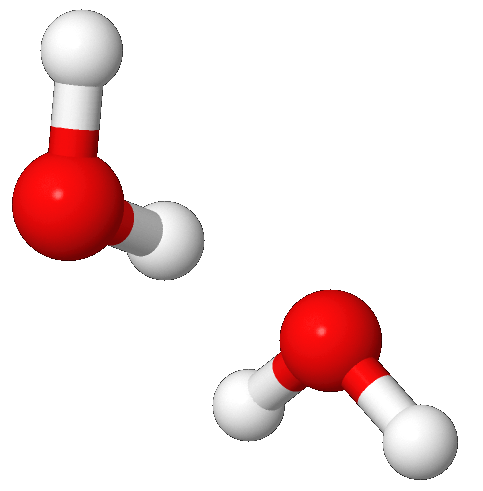
\includegraphics[width = 0.5\textwidth]{figures/h2o.png}
\caption{3D geometry of \hho\ dimer.}
\end{figure}

\begin{figure}
\centering
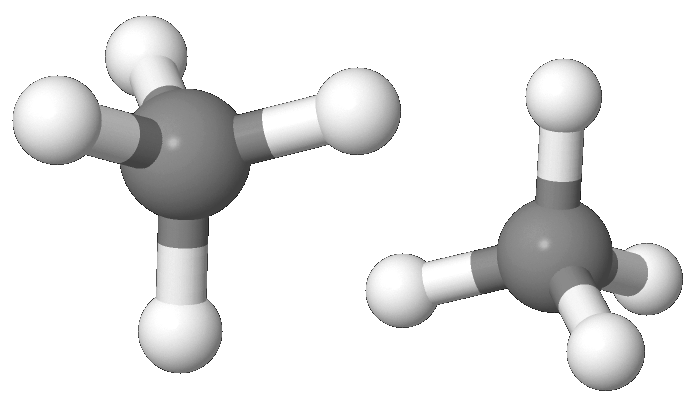
\includegraphics[width = 0.5\textwidth]{figures/ch4.png}
\caption{3D geometry of \ch\ dimer.}
\end{figure}

\begin{figure}
\centering
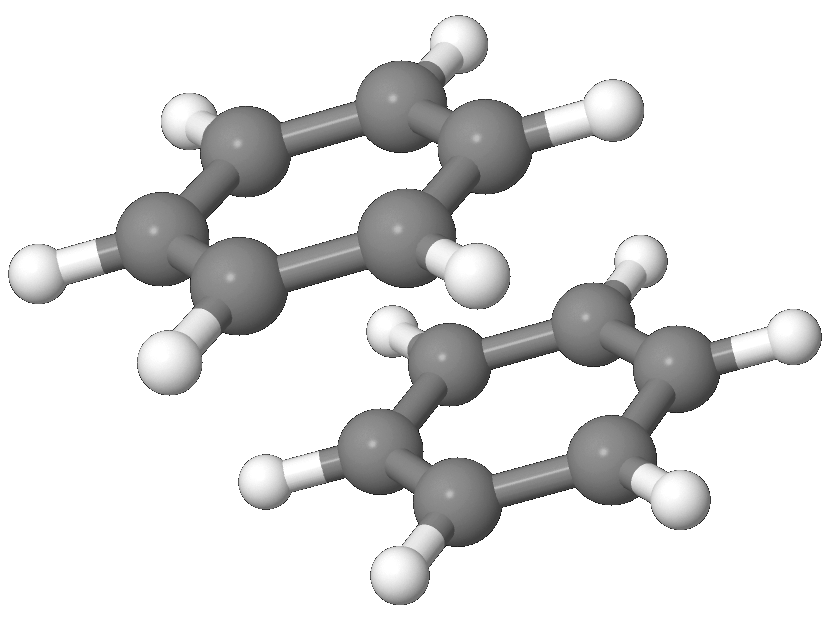
\includegraphics[width = 0.5\textwidth]{figures/benzene-parallel-displaced.png}
\caption{3D geometry of \benzpara\ dimer.}
\end{figure}

\begin{figure}
\centering
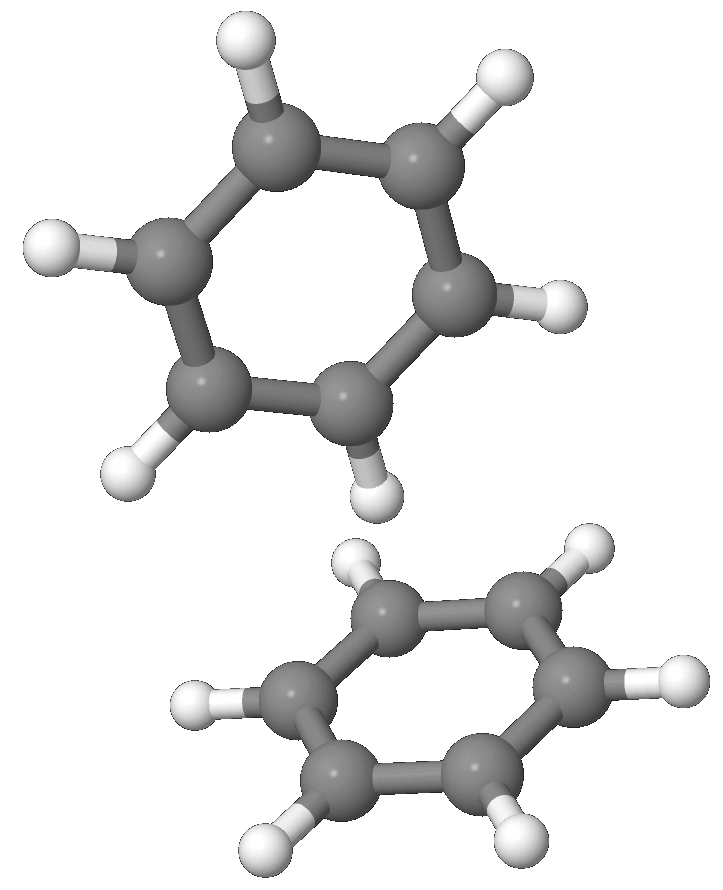
\includegraphics[width = 0.5\textwidth]{figures/benzene-T-shaped.png}
\caption{3D geometry of \benzT\ dimer.}
\end{figure}

\section{HF Calculations}

For each dimer system, the aug-cc-pVDZ basis set was used for HF and MC-MP2
calculations.

\section{MP2 Energies}

